\documentclass[10.5pt, aspectratio=169]{beamer} %handout

\usepackage{style}
%\usepackage[latin1]{inputenc}

\usepackage[style=authoryear,maxnames=2,backend=bibtex]{biblatex}
\addbibresource{bib_dpp_new.bib}

\setbeamertemplate{bibliography item}[text]

\usepackage{amsthm,amssymb}
\usepackage{amsmath}
\usepackage{mathtools}
\usepackage{graphicx}
\usepackage{hyperref}
\usepackage{amssymb}
\usepackage{caption}
\usepackage{listings}
\usepackage{subfig}
\usepackage{float}
\usepackage{bm}
\usepackage{color}
\usepackage{xcolor}
\usepackage{tikz}
\usetikzlibrary{tikzmark,calc,fit}


\usepackage{graphicx} %Loading the package
\graphicspath{{../images}}

\renewcommand{\div}{\text{div}}
\newcommand{\virgolette}[1]{``#1''}
\newcommand{\iid}{\stackrel{\mbox{\scriptsize iid}}{\sim}}
\newcommand{\ind}{\stackrel{\mbox{\scriptsize ind}}{\sim}}
\newcommand{\wtilde}{\widetilde{w}}
\newcommand{\mtilde}{\widetilde{m}}
\newtheorem{prop}{Proposition}


\newcommand{\Pp}{\mathbb{P}}
\newcommand{\X}{\mathbb{X}}
\newcommand{\Y}{\mathbb{Y}}
\newcommand{\E}{\mathbb{E}}


\newcommand{\calB}{\mathcal{B}}
\newcommand{\invWish}{\mathcal{IW}}
\newcommand{\Law}{\mathcal L}
\newcommand{\calU}{\mathcal U}
\newcommand{\ptilde}{\widetilde{p}}
\newcommand{\mutilde}{\widetilde{\mu}}
\newcommand{\dd}{\mathrm d}
\newcommand{\Ga}{\mbox{Gamma}}
\newcommand{\e}{\mathrm{e}}
\newcommand{\indicator}{\mathds{1}}
\newcommand{\Cov}{\mathrm{Cov}}

\newtheorem{proposition}{Proposition}

% \newcommand{\calN}{\mathcal{N}}
% \DeclareMathOperator{\Cov}{Cov}

\renewcommand{\footnotesize}{\scriptsize}
\DeclareMathOperator*{\argmin}{argmin} 

\usefonttheme{serif}

\title{Normalized Latent Measure \\ Factor Models}
\author{{\bf Mario Beraha}, Jim E. Griffin \\ University of Torino, University College London} 


\institute{BNP13, Puerto Varas}
\date{24 October 2022}



\begin{document}
\frame[plain]{

\titlepage

\begin{center}
Available at arXiv:2205.15654
\end{center}
}

% \begin{frame}{Presentation Plan}
%     \tableofcontents
% \end{frame}

%%%%%%%%%%%%%%%%%%%%%%%%%%%%%%%%%%
%%%%%%%%%%%%%%%%%%%%%%%%%%%%%%%%%%

% \section{Introduction}

%%%%%%%%%%%%%%%%%%%%%%%%%%%%%%%%%%
%%%%%%%%%%%%%%%%%%%%%%%%%%%%%%%%%%

\begin{frame}{Setup}

Observation \textbf{naturally grouped} into $g$ subpopulations
\[
	y_{11}, \ldots, y_{1n_1}, \ldots \ldots, y_{g1} \ldots, y_{g n_g}
\]

\only<2>{
\vspace{0.5cm}

\begin{columns}
\begin{column}{0.65\textwidth}
\textbf{Invalsi Dataset}
\bigskip
\begin{itemize}
	\setlength{\itemsep}{1.1em}
	\item Grades of a math test in Italian high schools, 40k students in $g > 1$k schools
	\item $4 \leq n_j \leq 140$
\end{itemize}
\end{column}

\begin{column}{0.35\textwidth}
\centering
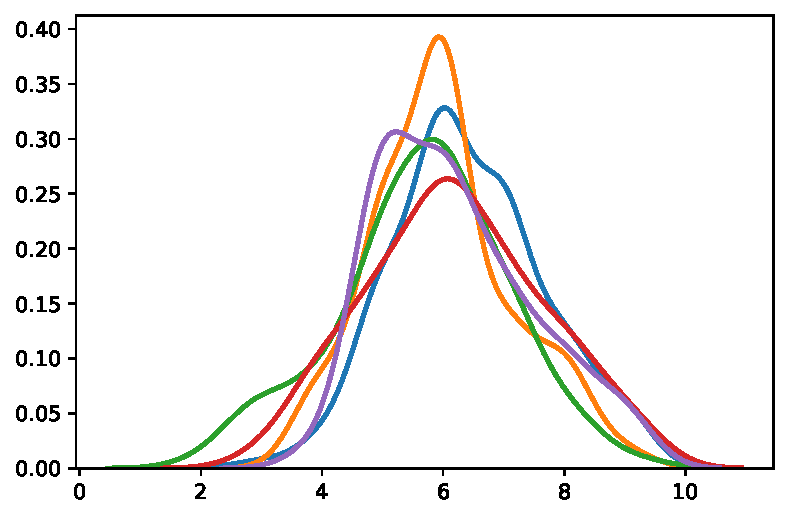
\includegraphics[width=0.95\linewidth]{example_invalsi}
\end{column}

\end{columns}
}

\only<3>{

\begin{columns}
\begin{column}{0.65\textwidth}
\textbf{Income Data in California}
\bigskip
\begin{itemize}
	\setlength{\itemsep}{1.1em}
	\item Fine spatial aggregation (PUMA level, 255 pumas)
	\item Take into account the spatial dependence
\end{itemize}
\end{column}

\begin{column}{0.35\textwidth}
\centering
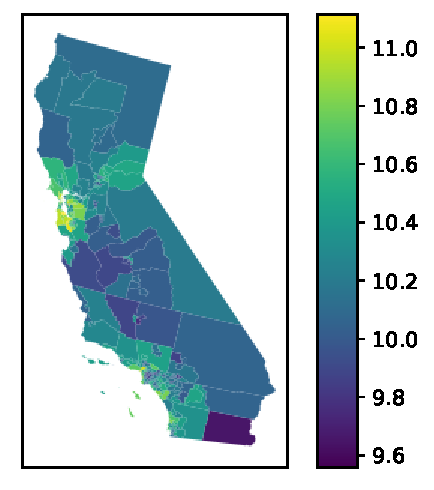
\includegraphics[width=0.95\linewidth]{example_income}
\end{column}

\end{columns}
}

\end{frame}


%\begin{frame}{Focus and goals}
%
%
%\textbf{Our typical setting}
%
%\vspace{0.3cm}
%
%\begin{columns}
%
%\begin{column}{0.6\textwidth}
%
%\begin{itemize}[<+->]
%	\item Focus \# 1: \textbf{density modelling} in each group 
%	
%	\item Few observations per group \\ $\Longrightarrow$ cannot inform \textbf{overparametrized} models
%	
%	\item Small differences across groups (mostly skewness)
%	
%	\item Focus \# 2: \textbf{explore} and \textbf{explain} the difference across groups 
%	
%	\item We are in a ``\emph{large $g$, small $n_j$ setting}''.
%
%\end{itemize}
%\end{column}
%
%\begin{column}{0.4\textwidth}
%
%\onslide<1-> {
%\begin{gather*}
%	y_{ji} \mid \ptilde_j \iid \int_\Theta f(\cdot \mid \theta) \ptilde_j(\dd \theta) \\
%	\ptilde_1, \ldots, \ptilde_g  \sim  \alert{Q}
%\end{gather*}
%}
%
%\onslide<2->{
%
%\vspace{-1cm}
%\begin{gather*}
%		Q(\dd \ptilde_1, \ldots, \dd \ptilde_g) \alert{\neq} \prod_{j=1}^g \mathrm{DP}(\dd \ptilde_j \mid \alpha G_0) \\
%		Q(\dd \ptilde_1, \ldots, \dd \ptilde_g) \only<2-3>{\textcolor{blue}{\stackrel{\mbox{?}}{\sim}}} \only<4->{\alert{\neq}} \mathrm{HDP}
%\end{gather*}
%}
%
%\end{column}
%\end{columns}
%\end{frame}


\begin{frame}{Focus and goals}


\begin{itemize}[<+->]
	\item Focus \# 1: \textbf{density modelling} in each group 
\begin{equation*}
	y_{ji} \mid \ptilde_j \iid \int_\Theta f(\cdot \mid \theta) \ptilde_j(\dd \theta), \qquad
	\ptilde_1, \ldots, \ptilde_g  \sim  \alert{Q}
\end{equation*}
	
	\item Few observations per group: ``\emph{large $g$, small $n_j$ setting}''. \\ $\Longrightarrow$ cannot inform \textbf{overparametrized} models
		
	
	\begin{equation*}
		Q(\dd \ptilde_1, \ldots, \dd \ptilde_g) \alert{\neq} \prod_{j=1}^g \mathrm{DP}(\dd \ptilde_j \mid \alpha G_0), \qquad 
		Q(\dd \ptilde_1, \ldots, \dd \ptilde_g) \only<1-2>{\textcolor{blue}{\stackrel{\mbox{?}}{\sim}}} \only<3->{\alert{\neq}} \mathrm{HDP}
	\end{equation*}

	
	\item Focus \# 2: \textbf{explore} and \textbf{explain} the difference across groups 
	
\end{itemize}
\end{frame}

\begin{frame}{Practical Example: California Income Data}

\only<1>{
\begin{center}
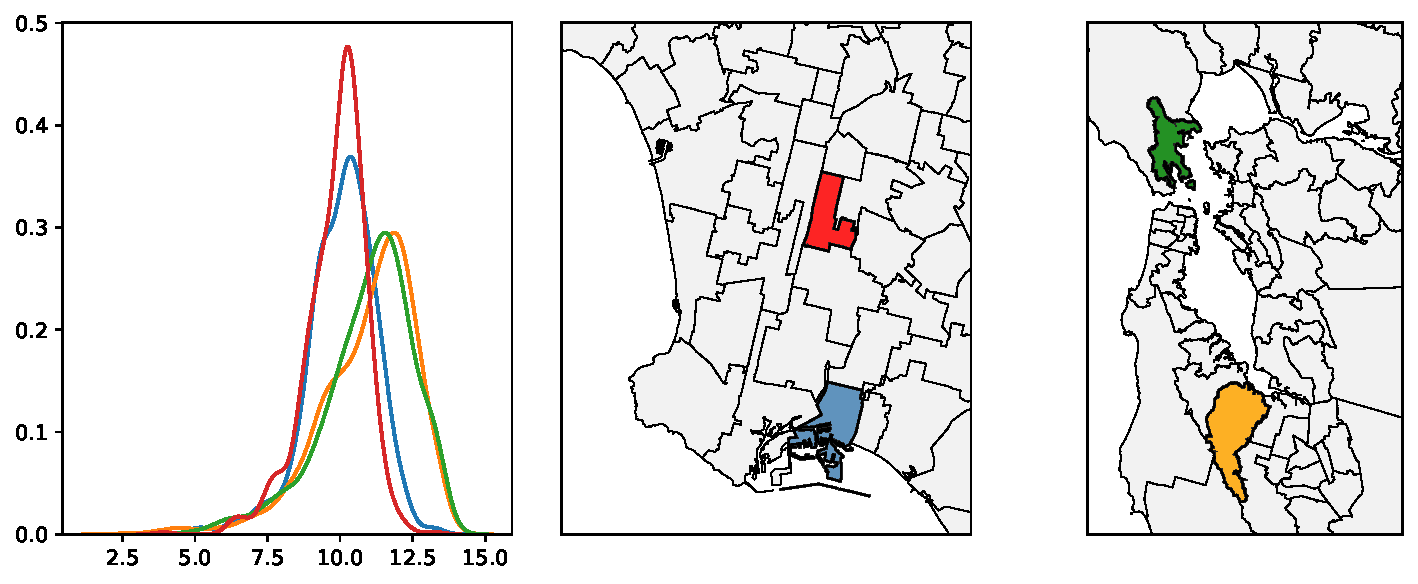
\includegraphics[width=0.8\linewidth]{four_pumas}
\end{center}
}

\only<2-3>{
	\centering
	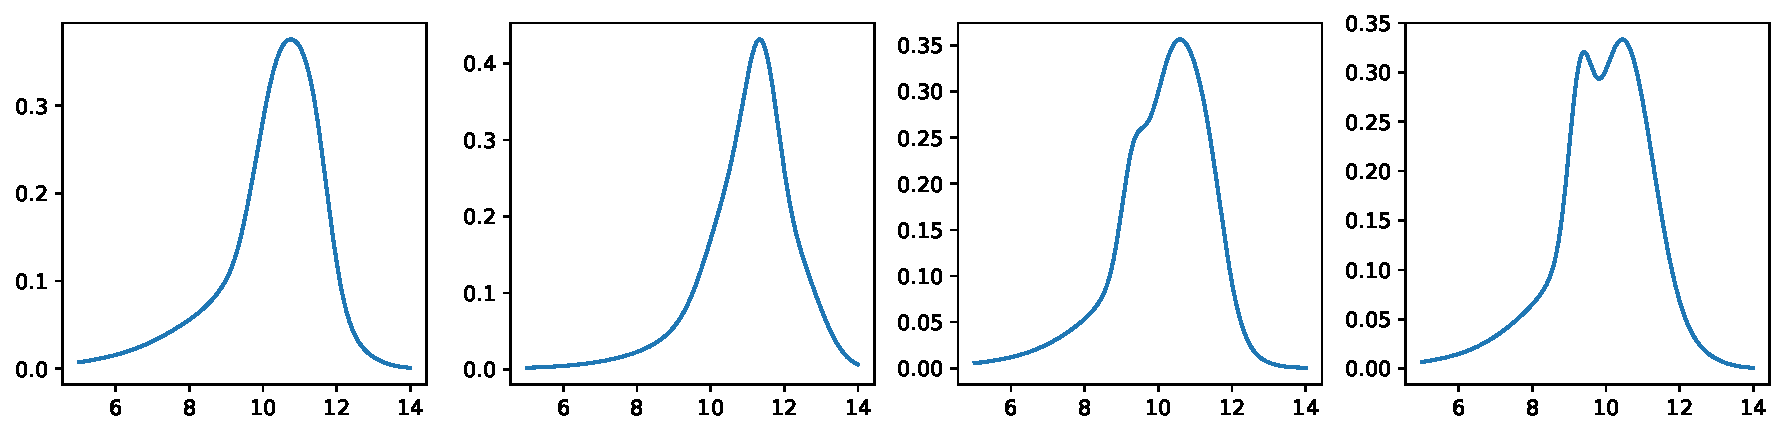
\includegraphics[width=0.9\linewidth]{income_latent_factors}
}

\only<3>{
\centering
\hspace{1cm} 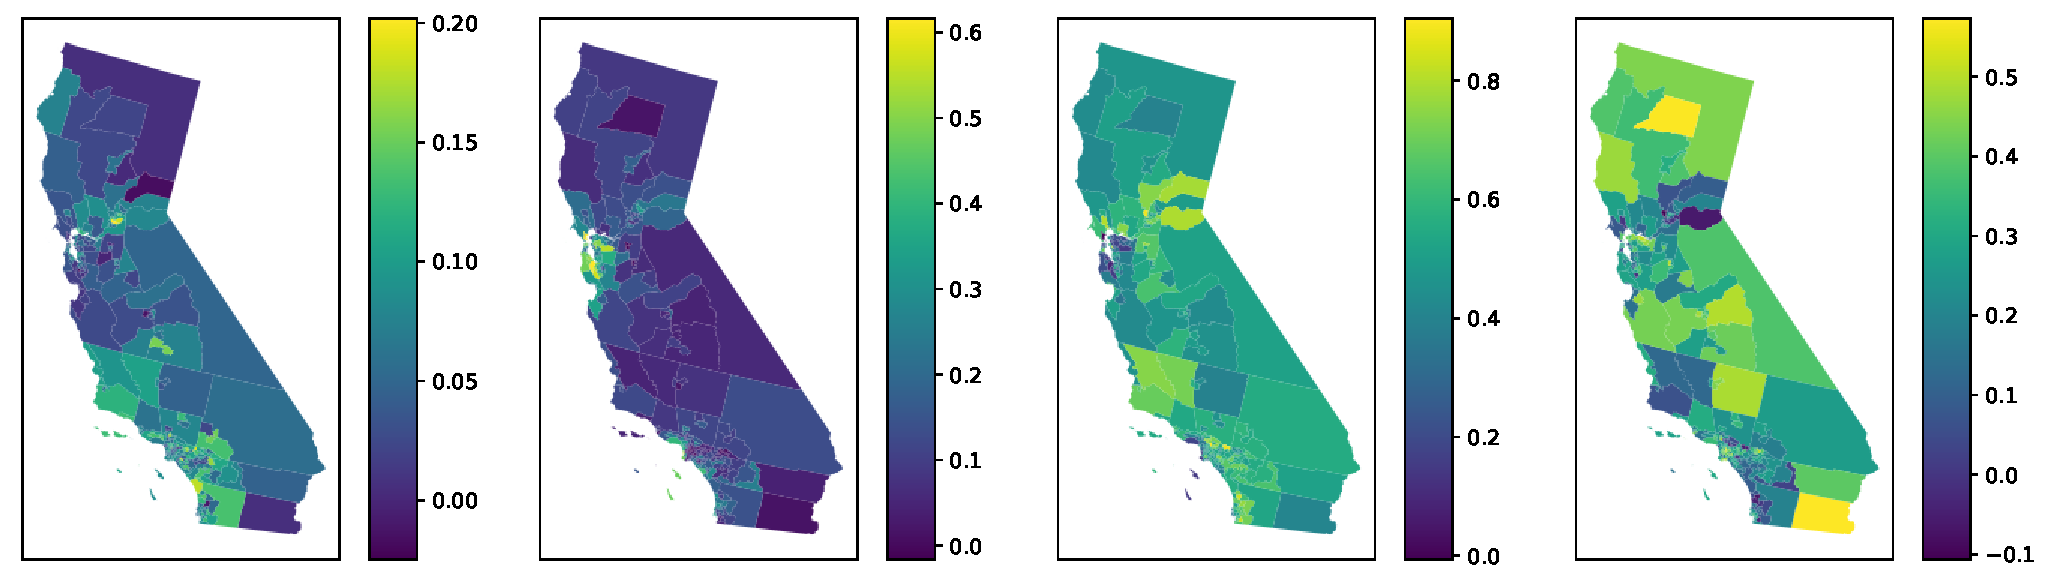
\includegraphics[width=0.9\linewidth]{income_lam}
}





\end{frame}



\begin{frame}{Latent Factor Models}
	
	\begin{center}
		\emph{large $g$, small $n_j$} \quad $\approx$ \quad \emph{large $p$, small $n$}
	\end{center}
	
	\onslide<2->{
		$x_1, \ldots, x_n \in \mathbb{R}^p$, $p \gg n$.
		
		\begin{equation*}
			\begin{aligned}
				x_i \mid  \Lambda,\eta_i & \ind \calN_p(\Lambda \eta_i, \Sigma) \only<3>{\\
				\eta_1, \ldots, \eta_n & \iid \calN_H(0, I), \quad H \ll p \\
				\Lambda \sim \pi(\Lambda) \quad & \qquad \Sigma \sim \pi(\Sigma)}
			\end{aligned}
		\end{equation*}
	}
	
	\onslide<4->{
	\begin{itemize}
		\item \textbf{Parsimonious} model
		\item \textbf{Interpretability} of latent factors (\emph{main variability}) and loadings
	\end{itemize}
	
	}
	
	\onslide<5->{
		\[
			x_{ij} = \sum_{h = 1}^H \lambda_{jh} \eta_{ih} + \varepsilon_{ij}, \ j=1, \ldots, p \onslide<6-> \quad \Longrightarrow \quad \ptilde_j = \sum_{h=1}^H \lambda_{jh} p^*_h, \ j=1, \ldots, g
		\]
	}

\end{frame}




\begin{frame}{A Normalized Random Measure Approach}

\only<1-2>{
\[
	y_{ji} \mid \ptilde_j \iid \int_\Theta f(\cdot \mid \theta) \ptilde_j(\dd \theta), \quad i=1, \ldots, n_j
\]

	Avoid overly constrained parameters by setting
}	
	\begin{align*}
		\ptilde_j = \frac{\mutilde_j}{\mutilde_j(\Theta)} , \qquad
		\mutilde_{j} = \sum_{h=1}^H \lambda_{jh} \mu^*_h
	\end{align*}

\only<2>{
	\begin{itemize}
		\item $\lambda_{jh}$'s must be positive
		\item $\mu^*_1, \ldots, \mu^*_H$ a collection of completely random measures
	\end{itemize}
}
	
\only<3>{
Connections with normalized \textbf{additive processes}

\begin{itemize}[<+->]
	\setlength{\itemsep}{1.1em}
	\item Lijoi et al. (2014): $g=2$, $H=3$, $\lambda_1 = (1, 1, 0)$, $\lambda_2 = (1, 0, 1)$ \\
	$\Longrightarrow$ focus on flexible sharing of information 
	\item Griffin et al. (2013): $g > 2$, $H = 2^g$ (typically), $\lambda_{jh} \sim \mbox{Bern}(\rho)$ \\
	$\Longrightarrow$ focus on detecting the presence of differences
	\item No way of extracting ``characteristic traits'' across populations
\end{itemize}

}

\end{frame}


\begin{frame}{Prior Modelling -- the $\mu^*_h$'s}
Most natural choice
	\[
		\mu^*_h = \sum_{k \geq 1} J_{hk} \delta_{\theta_{hk}} \iid \mathrm{CRM}(\nu_h; \Theta)
	\]


\onslide<2->{Still too many parameters! No need for measure-specific atoms}

\bigskip

\onslide<3->{Compound Random Measures (CoRMs; Griffin and Leisen, 2017)
\[
	\mu^*_h = \sum_{k \geq 1} m_{hk} J_k \delta_{\theta^*_k}
\]
}
\onslide<4->{
Default choice:
\[
	m_{hk} \iid \mbox{Gamma}(\phi, 1)
\]
}
\onslide<5->{
Marginally, each $\mu^*_h$ is a Gamma process with base measure $\alpha(\dd \theta)$.
}
\end{frame}


\begin{frame}{A fresh take on the model}

When $\mu^*_1, \ldots, \mu^*_H \sim \mbox{CoRM}$, we have
\[
	\mutilde_j = \sum_{k \geq 1} \only<1>{\alert{(\Lambda M)_{jk}}} \only<2->{\alert{\Gamma_{jk}}} J_k \delta_{\theta_k}
\]


\onslide<2->{

\begin{itemize}
	\setlength{\itemsep}{1.2em}
	\item Essentially, forcing a parsimonious factorization of the matrix $\Gamma \approx \Lambda M$
	\item Connections to Nonnegative Matrix Factorization and Independent Component Analysis!
\end{itemize}
}

\end{frame}


\begin{frame}{Prior Modelling -- the matrix $\Lambda$, Invalsi dataset}

\begin{itemize}[<+->]
	
	\item No additional group-specific information
	
	\item Very large number of groups $\Longrightarrow$ impractical to choose $H$ via model selection
	
	\item \alert{Multiplicative Gamma Process} (Bhattacharya and Dunson, 2011) for $\Lambda$:
	\[
		\lambda_{jh} = (\phi_{jh} \tau_h)^{-1}, \qquad \tau_{h} = \prod_{j=1}^h \theta_j,	
	\]
	\[
		\theta_1 \sim \mbox{Ga}(a_1, 1), \ \  \theta_2, \ldots \iid  \mbox{Ga}(a_2, 1), \quad  \phi_{jh} \iid  \mbox{Ga}(\nu/2, \nu/2)
	\] 
	
	\item Learn $H$ through adaptive Gibbs sampling in the first MCMC iterations
\end{itemize}
\end{frame}



\begin{frame}{Prior Modelling -- the matrix $\Lambda$, California Income}

\begin{columns}
\begin{column}{0.65\textwidth}

Known neighboring relation between areas $i \sim j$.

\begin{itemize}
	\item log-Gaussian Markov Random Field prior for $\Lambda$ (by column)
	\[
		\log \bm \lambda^h \iid \mathcal{N}_H\left(\mu, \left(\tau (F - \rho G)\right)^{-1}\right)
	\]
	$G_{ij} = 1$ if and only if $i \sim j$, $F_{ii} = \sum_{j} G_{ij}$.
	
	\item Poor mixing when $\tau$ is random
	
	\item Poor scalability when $\rho$ is random
\end{itemize}

\end{column}

\begin{column}{0.35\textwidth}
\centering
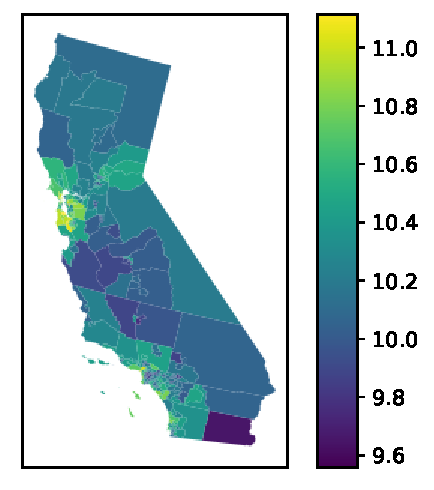
\includegraphics[width=0.95\linewidth]{example_income}
\end{column}

\end{columns}

\pause

\vspace{0.5cm}

Choose $H$ via model selection.

\end{frame}



\begin{frame}{Posterior Inference}

\begin{itemize}
	\setlength{\itemsep}{1.1em}
	\item No close form expression of the marginal distribution or the posterior
	\item MCMC via slice sampling or \textbf{a priori truncation}
	\item Sampling of $\Lambda$ and $M$ via Hamiltonian Monte Carlo
\end{itemize}

\pause

\bigskip
We want to \textbf{interpret}
\begin{itemize}
	\setlength{\itemsep}{1.1em}
	\item $\int_{\Theta} f(\cdot \mid \theta) \mu^*_h(\dd \theta)$ (possibly after normalization) as the $H$ \emph{common traits}
	\item The matrix $\Lambda$ in light of the common traits
\end{itemize}
\end{frame}



\begin{frame}{Non-indentifiability}

Recall
\vspace{-0.5cm}
\[
	\mutilde_j = \sum_{h=1}^H \lambda_{jh} \mu^*_h = \sum_{k \geq 1} (\Lambda M)_{jk} J_k \delta_{\theta^*_k}
\]

Posterior samples from $\int_{\Theta} f(\cdot \mid \theta) \mu^*_h(\dd \theta)$ in a simulated example

\begin{center}
	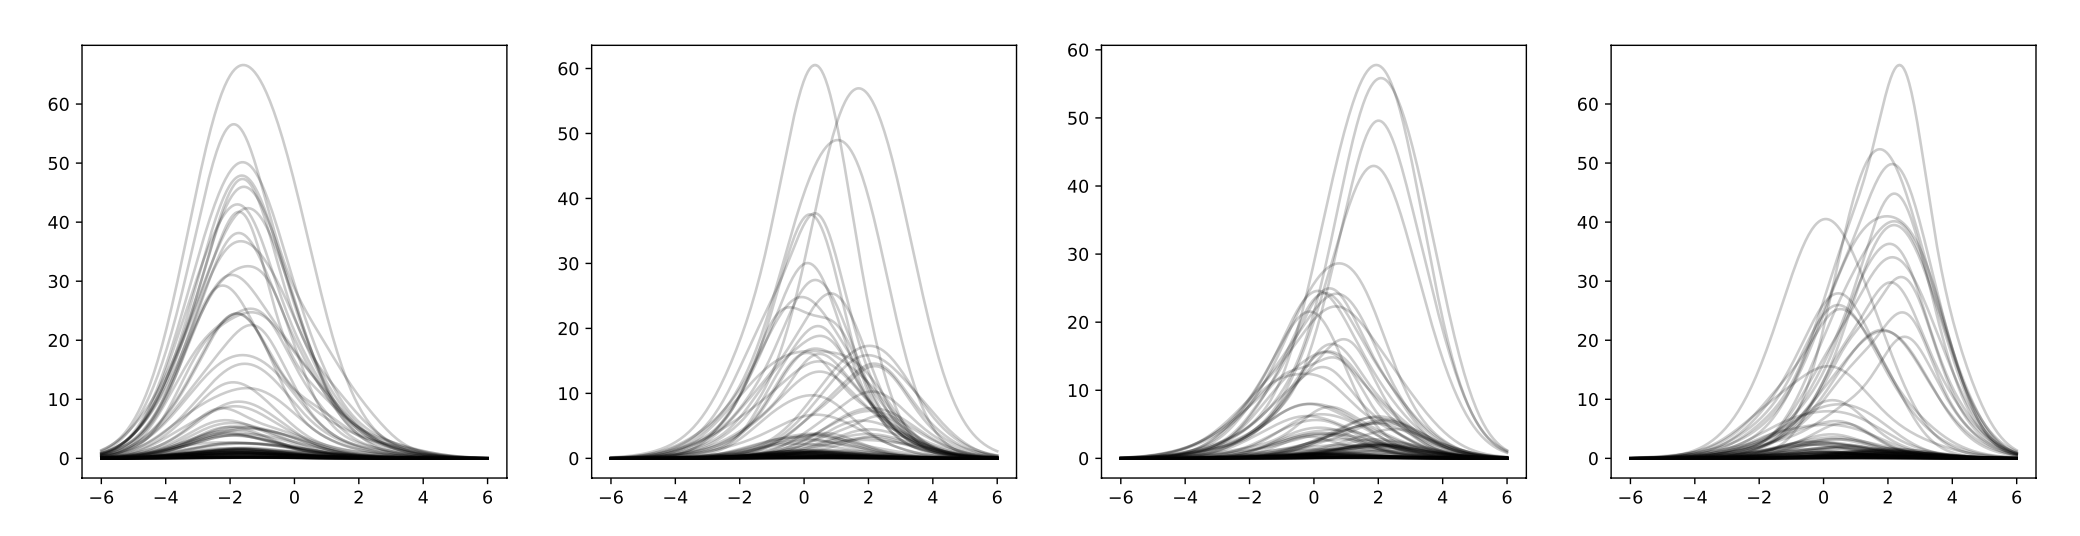
\includegraphics[width=0.8\linewidth]{latent_factors_before}
\end{center}

\onslide<2->

Sources of non-identifiability

\begin{itemize}
	\item	For all invertible $Q$, $\Lambda^\prime = \Lambda Q^{-1}$, $M^\prime = Q M$ \onslide<4->{\alert{$\Longrightarrow$ find optimal $Q$}}
	\item Label switching of the latent measures \onslide<4->{\alert{$\Longrightarrow$ optimal matching to a template}}
\end{itemize}

\onslide<3->

We follow Poworoznek et al. (2021) and propose a post-processing algorithm

\end{frame}


\begin{frame}{Learning an optimal $Q$ -- What to look for?}

We optimize an ``interpretability criterion''. Let $p^\prime_j(y) =  \sum_{k} (QM)_{ jk} J_k f(y \mid \theta_k)$
\[
	Q^* = \argmin \mathcal L(Q; \mu^*, f) = \sum_{j, \ell} \langle  p^\prime_j,  p^\prime_\ell \rangle
\]


\begin{itemize}
	\item $\langle f, g \rangle$ is the $L_2$ inner product
	\item low values of $\mathcal L$ correspond to densities with little overlap
\end{itemize}
\end{frame}


\begin{frame}{Learning an optimal $Q$ -- Where to look for?}

\textbf{Constraints}
\[
	QM \geq 0, \qquad \Lambda Q^{-1} \geq 0
\]

\pause

\medskip

$Q^{-1}$ must exist!

\pause 

\medskip

We don't want too extreme values in $Q$

\pause

\[
	Q^* = \argmin_{Q \in SL(H)} \mathcal L(Q; \mu^*, f) 
\]

$SL$ is the special linear group: matrices with determinants equal to 1

\end{frame}


\begin{frame}{Learning an optimal $Q$ -- How to look for it?}

$SL$ is a Riemannian manifold. We can design a gradient descent algorithm that stays always inside $SL$.

\medskip

\begin{columns}
\begin{column}{0.7\textwidth}

Basic version (Riemannian gradient descent):
\[
	Q_{n+1} = Q_n \exp\left( - h \partial_Q \mathcal L \right), \qquad \partial_Q \mathcal L = (\nabla \mathcal L)^\top
\]

\onslide<2->{

\bigskip
Deal with $QM \geq 0$, $\Lambda Q^{-1} \geq 0$ using an augmented Lagrangian multiplier method
\[
	\mathcal L_\rho(Q, \gamma) = \mathcal L(Q; M, J, \theta) + \frac{\rho}{2} \sum_j \max\left\{0, \frac{\gamma_j}{\rho} c_j(Q) \right\}
\]
}
\onslide<3->{

Alternate optimizing w.r.t. $Q$ and w.r.t. $\gamma_j$, $\rho$.
}
\end{column}

\begin{column}{0.3\textwidth}
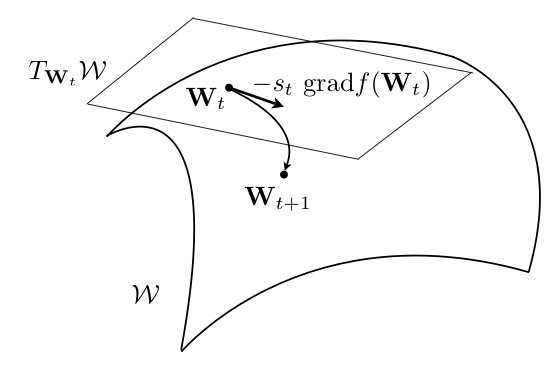
\includegraphics[width=\linewidth]{rgd}
\end{column}

\end{columns}
\end{frame}

\begin{frame}{Solving the Label-Switching}

As in Poworoznek et al. (2021), we choose a template $\hat \mu_1, \ldots, \hat \mu_H$ and align all samples to it.

\pause
\[
	\inf_{P \in \text{Perm}_H} \sum_{h, k=1}^H d(\hat \mu_h, \mu^{(j)}_k) P_{hk}
\]

\pause
Efficiently solved through Optimal Transport (cf. Birkhoff's theorem)
\pause
\[
	d(\hat \mu_h, \mu^\prime_j) = \Big \|  \hat \mu_h(\Theta)^{-1} \int_\Theta f(y \mid \theta) \hat \mu_h(\dd \theta)  - \mu^\prime_j(\Theta)^{-1} \int_\Theta f(y \mid \theta) \mu^\prime_j(\dd \theta) \Big\|
\]
\pause
or
\[
	d(\hat \mu, \mu^\prime)^2 = \inf_{T \in \Gamma(\hat \mu, \mu^\prime)} \sum_{h, k=1}^K W^2_2(f(\cdot \mid \hat \theta_h), f(\cdot \mid \theta^\prime_k))  T_{hk}
\]

\end{frame}


\begin{frame}{A Simulated Example}

100 groups from
\[
	y_{j, i} \iid  w_{j1} \calN(-2, 2) +  w_{j2} \calN(0, 2) +  w_{j1} \calN(2, 2), \qquad \bm w_j  \iid \mbox{Dirichlet}(1, 1, 1)
\]

\centering
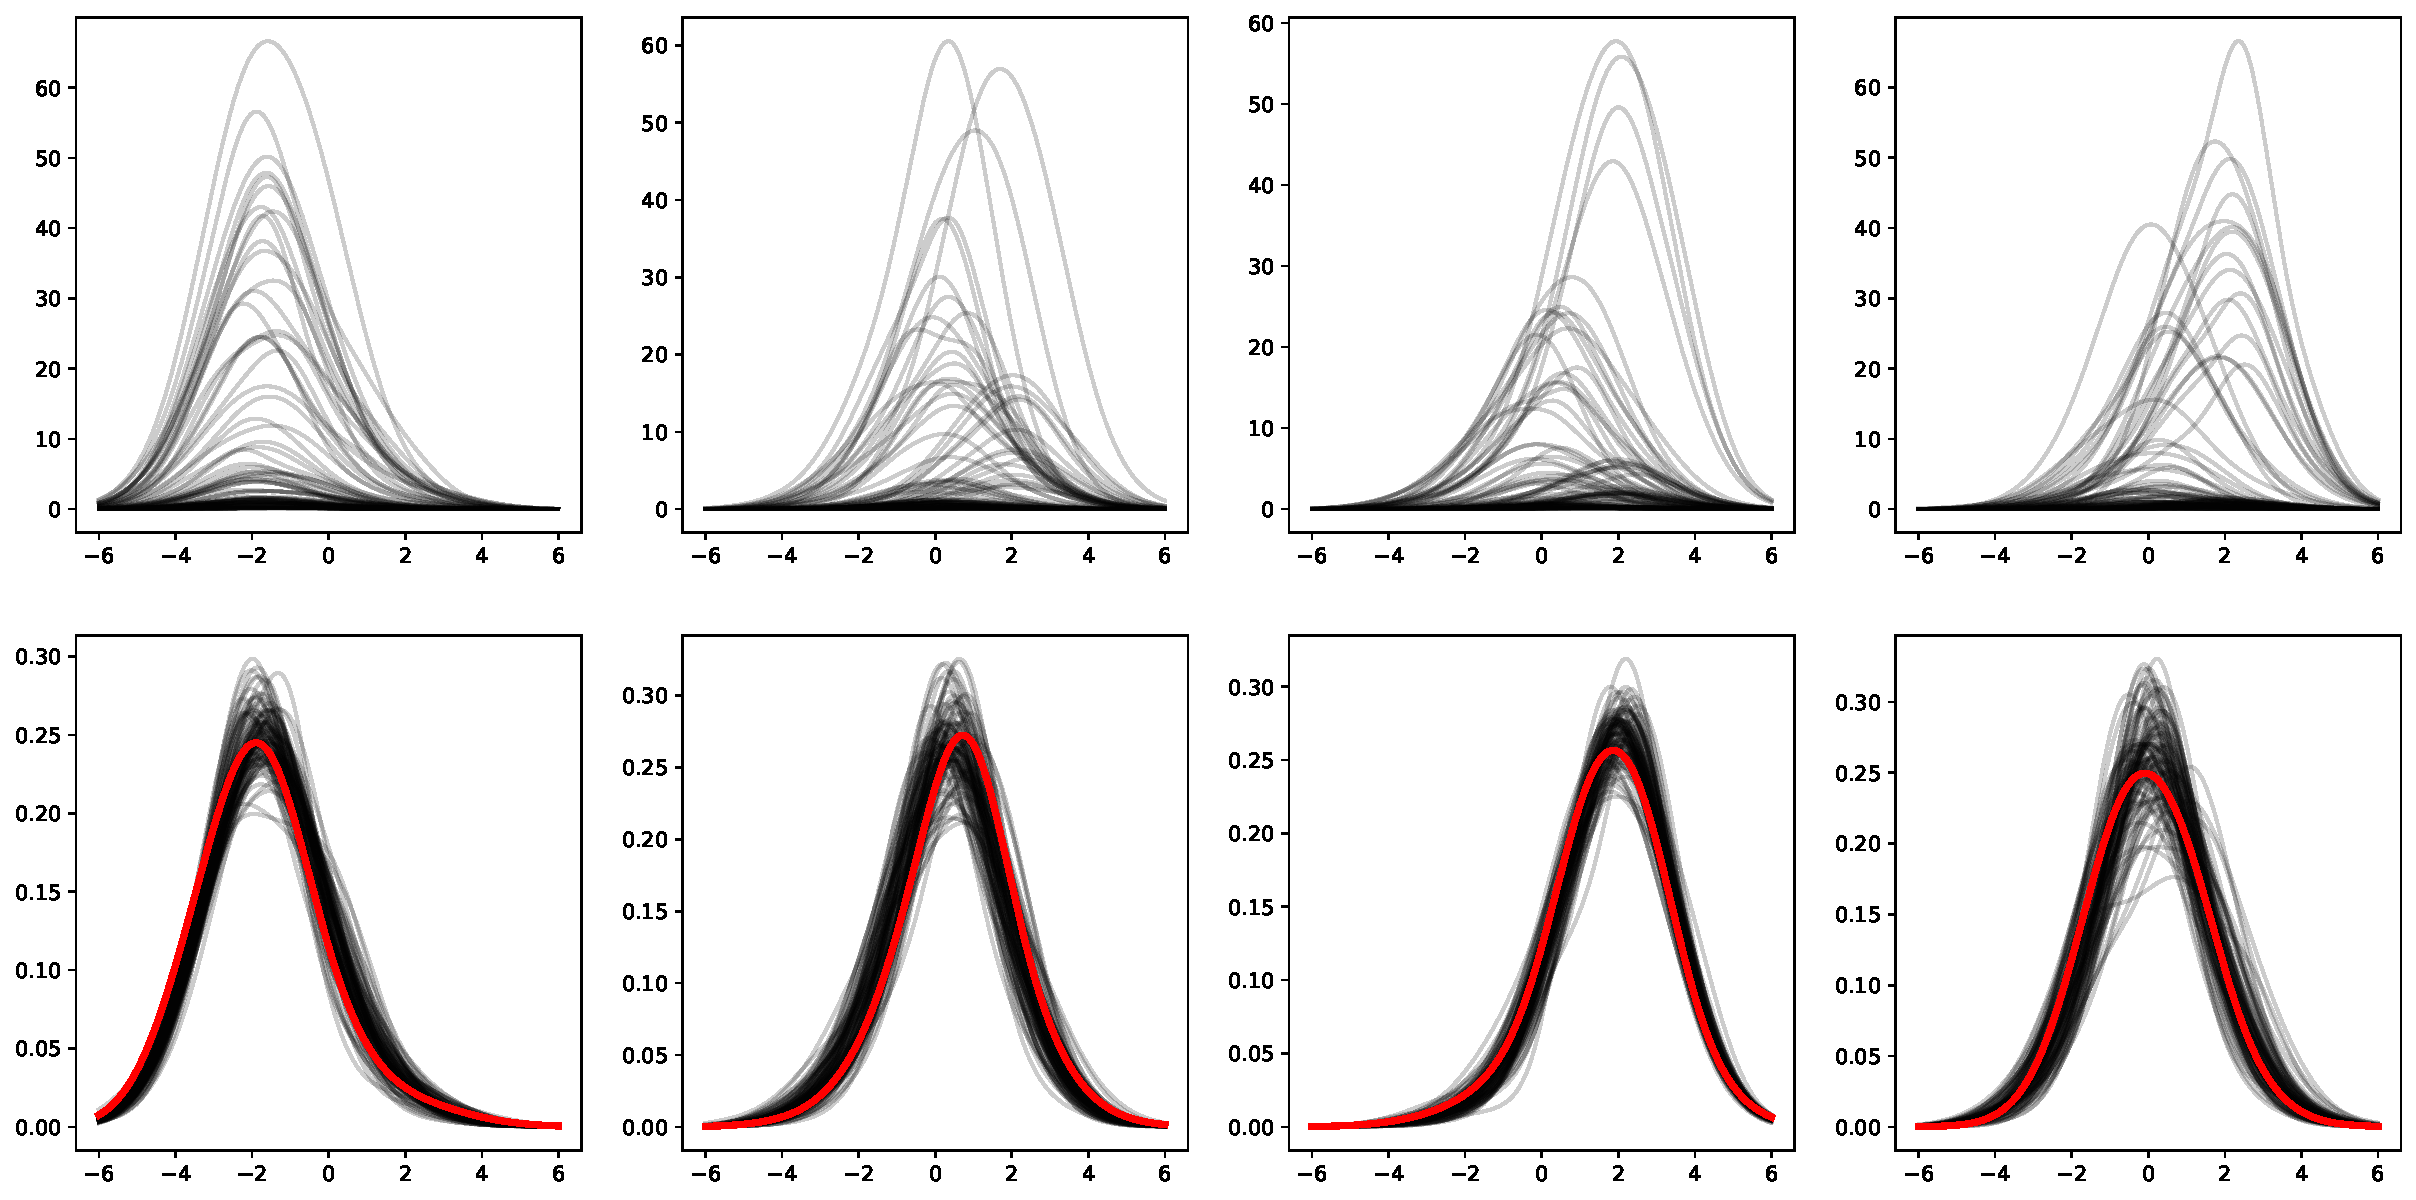
\includegraphics[width=0.7\linewidth]{simu_mgp_latent_dens}


\end{frame}


\begin{frame}{The Invalsi Dataset}

Grades of a math test in Italian high schools, 40k students in $g > 1$k schools.

\bigskip

\only<1>{

The latent measures

\centering
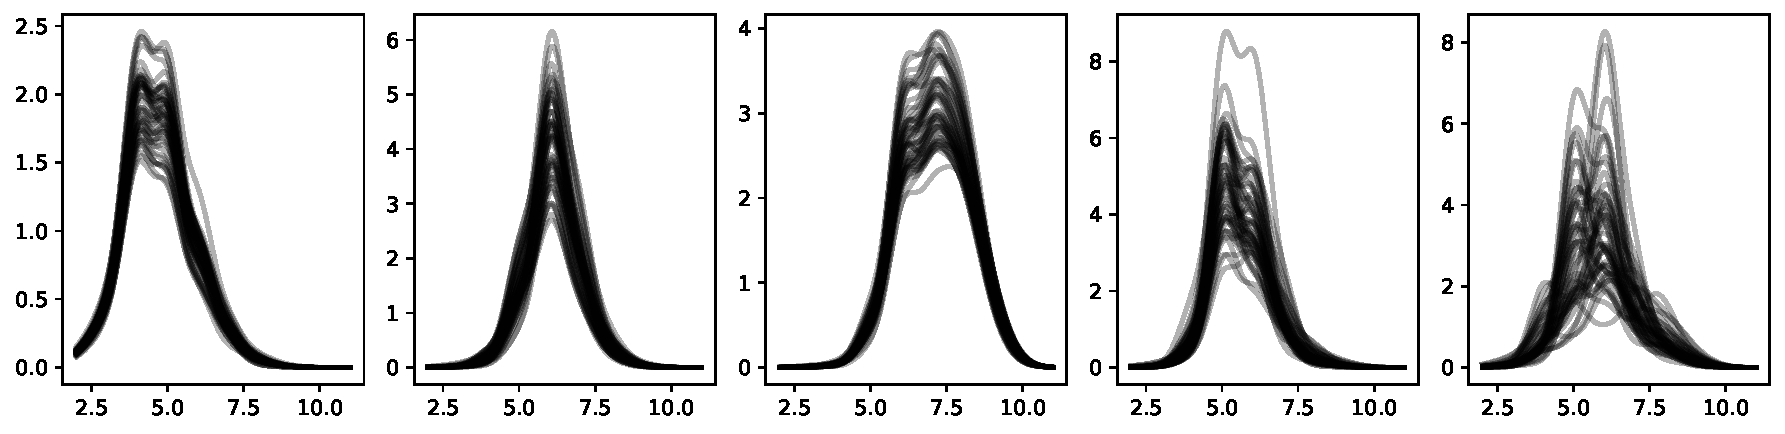
\includegraphics[width=0.9\linewidth]{invalsi_latent_draws}
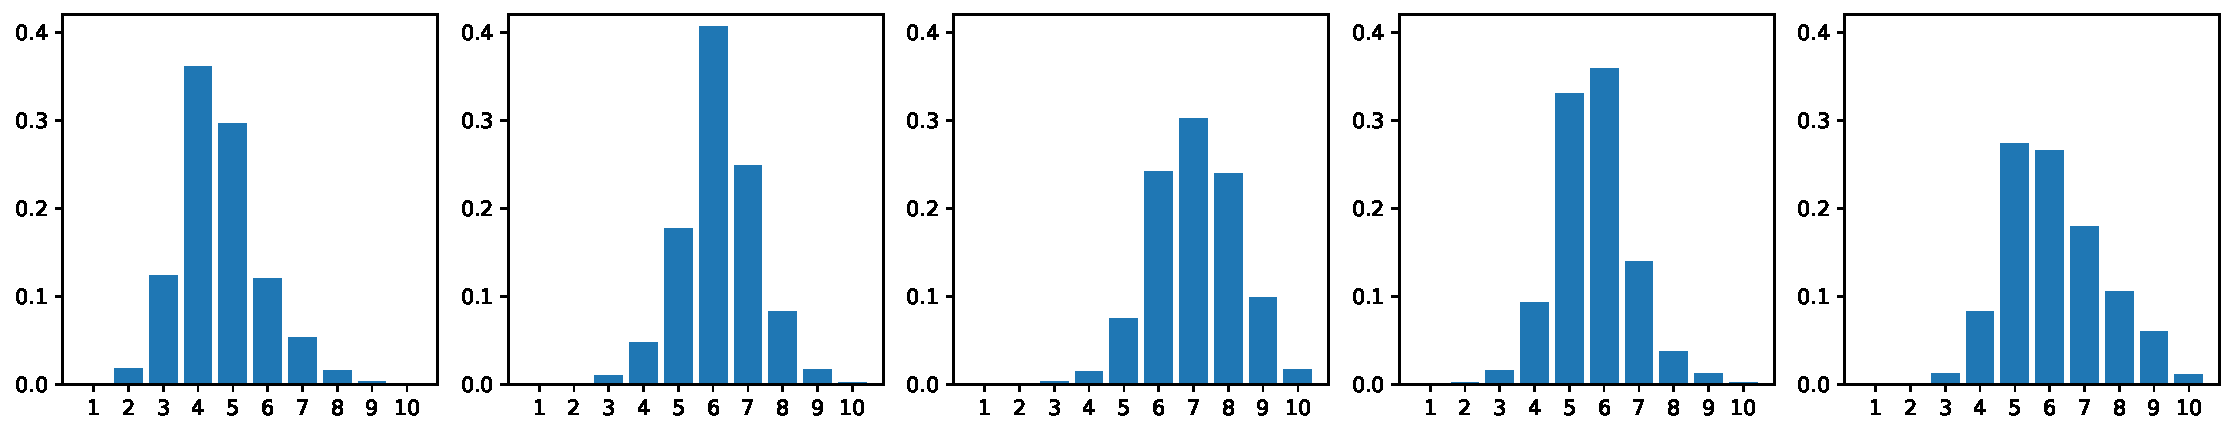
\includegraphics[width=0.9\linewidth]{invalsi_latent_factors_discrete}
}

\only<2>{

Clustering $\Lambda$'s rows

\centering
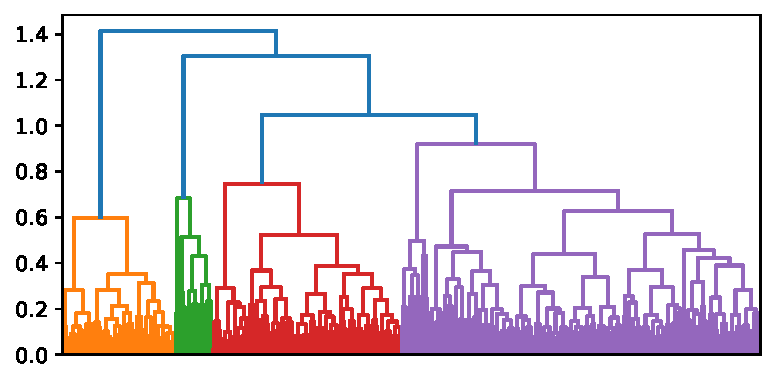
\includegraphics[width=0.4\linewidth]{invalsi_hclust_complete}
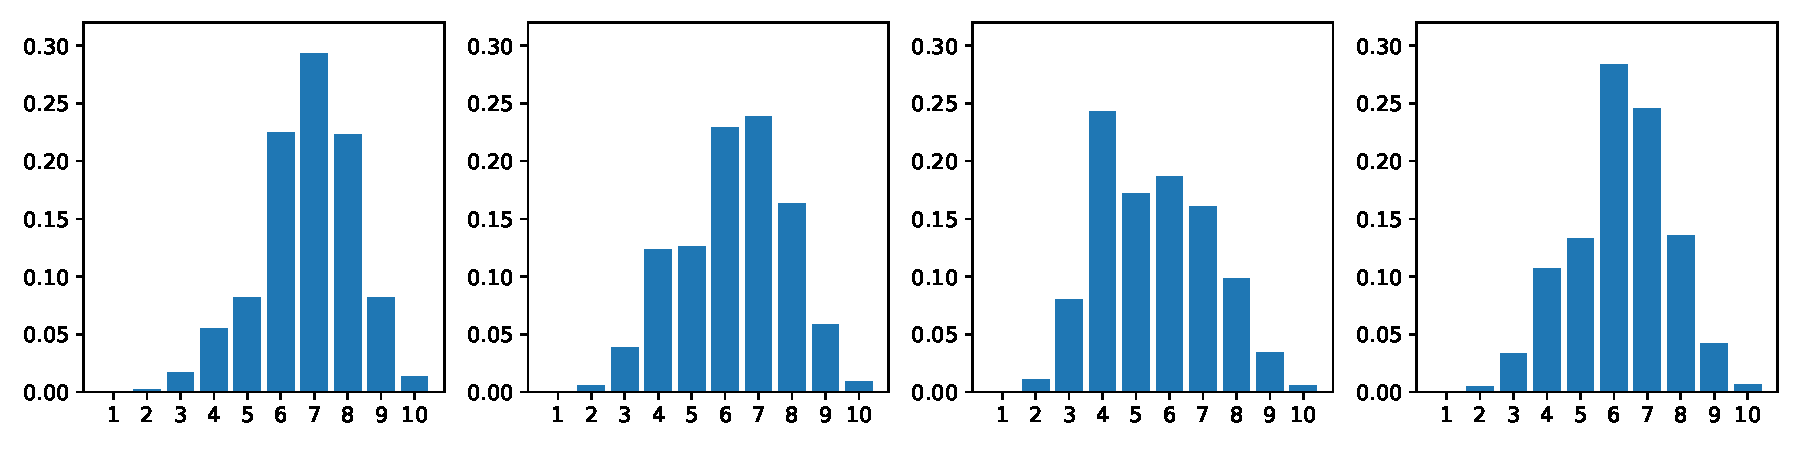
\includegraphics[width=0.9\linewidth]{invalsi_cluster_dens_discrete}
}

\end{frame}


\begin{frame}{US Income Data}

Personal income in $g > 250$ PUMAs in California

\only<1-2>{
\centering
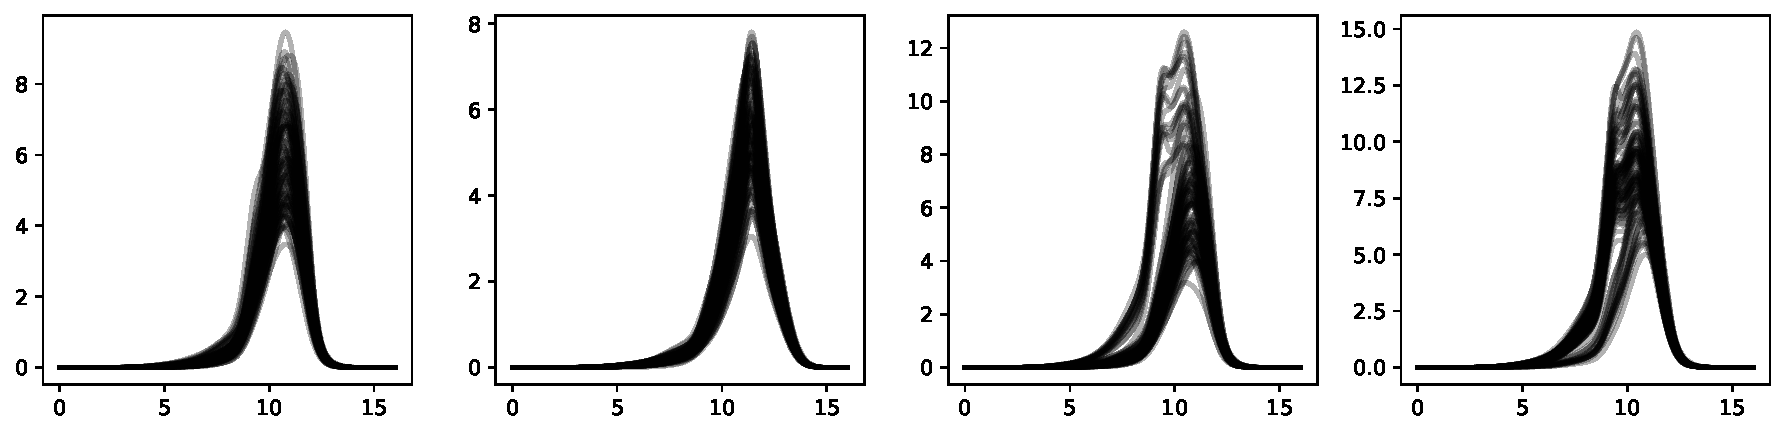
\includegraphics[width=0.9\linewidth]{income_latent_draws}
}
\only<2-3>{
\centering
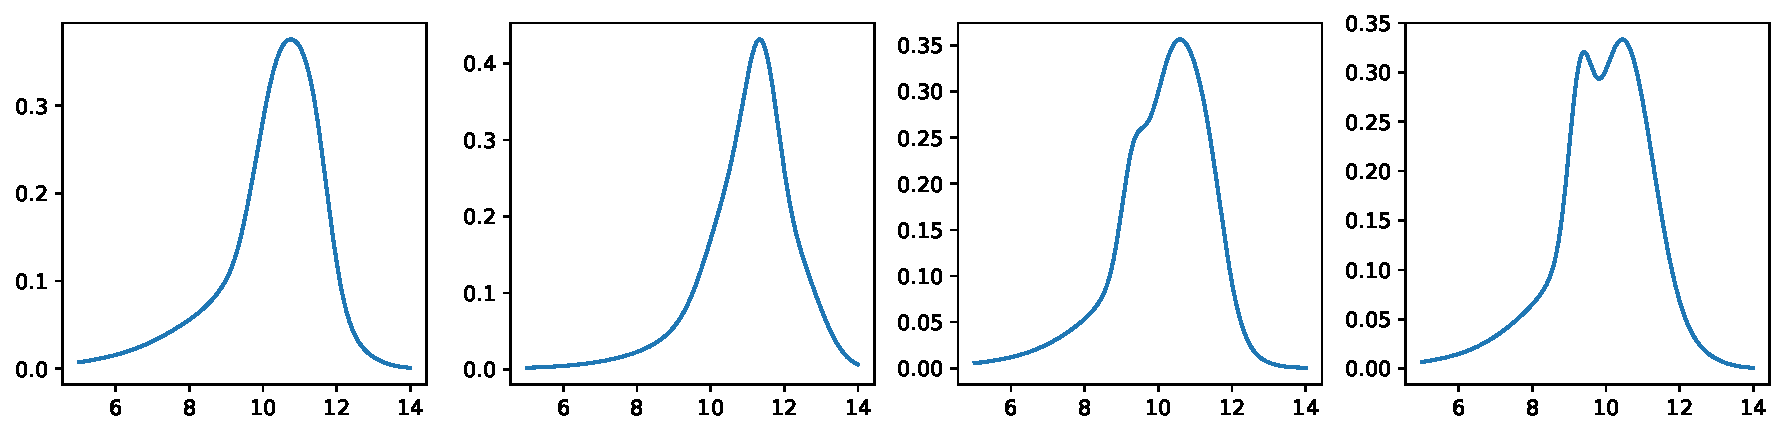
\includegraphics[width=0.9\linewidth]{income_latent_factors}
}
\only<3-4>{
\[
	p_j = \int_\Theta f(\cdot \mid \theta) \bar{\ptilde}(\dd \theta) + \sum_{h=1}^H s_{jh} \int_\Theta  f(\cdot \mid \theta) \epsilon_h(\dd \theta)
\]
where $ \bar{\ptilde}$ is the \textbf{overall mean measure} and the $\epsilon_h$ are the \textbf{residual measures}.
}

\only<4->{
\centering
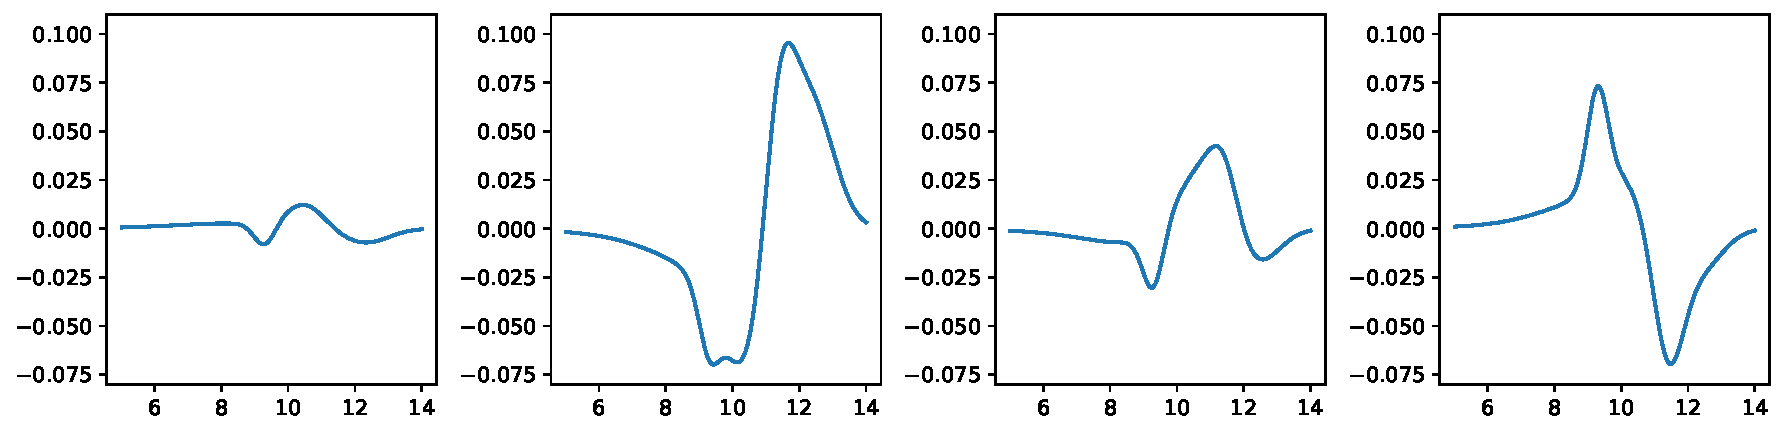
\includegraphics[width=0.9\linewidth]{income_latent_factors_diff}
}
\only<5>{
\centering

\hspace{1cm} 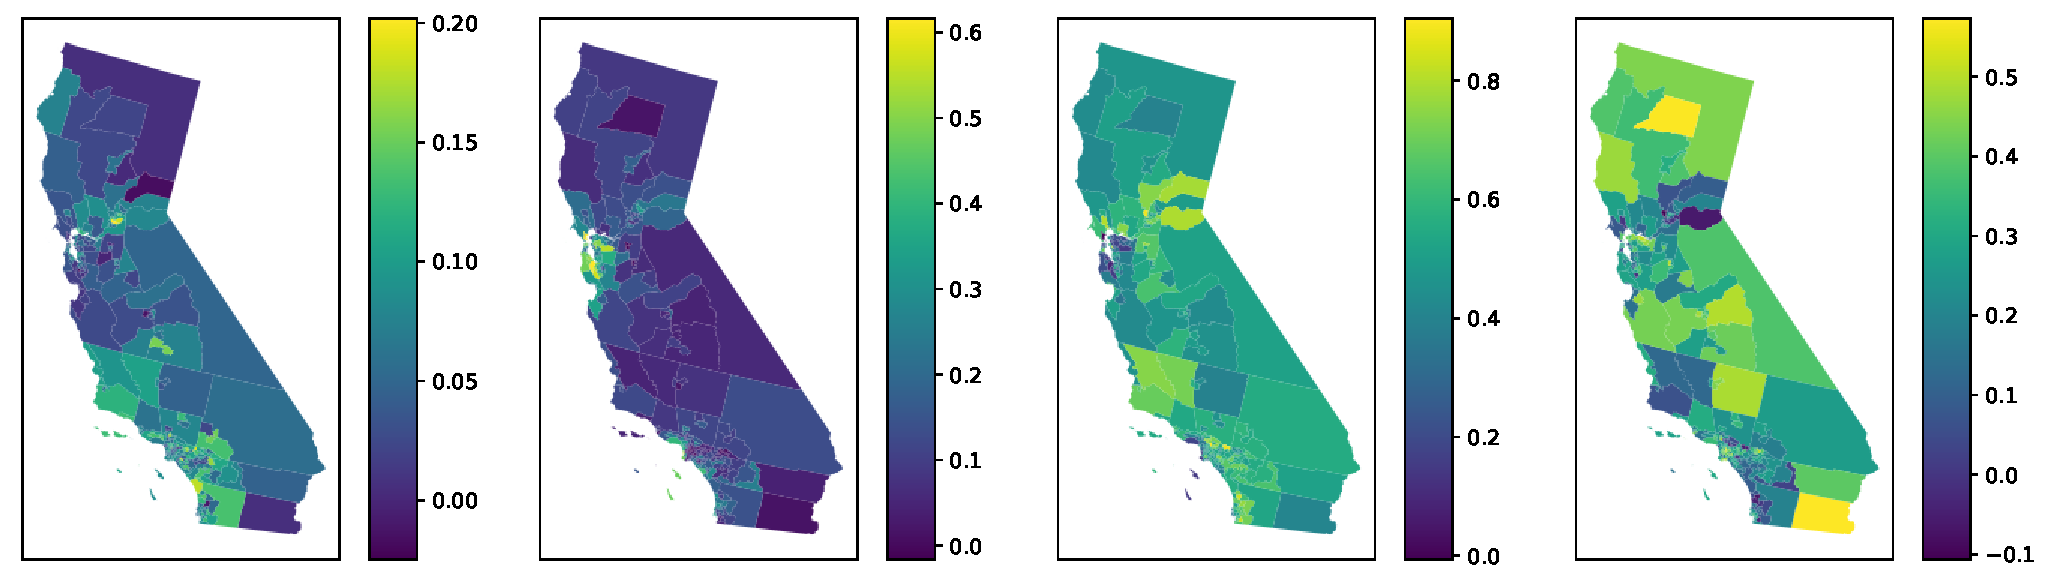
\includegraphics[width=0.9\linewidth]{income_lam}
}
\only<6>{
\centering

\hspace{1cm} 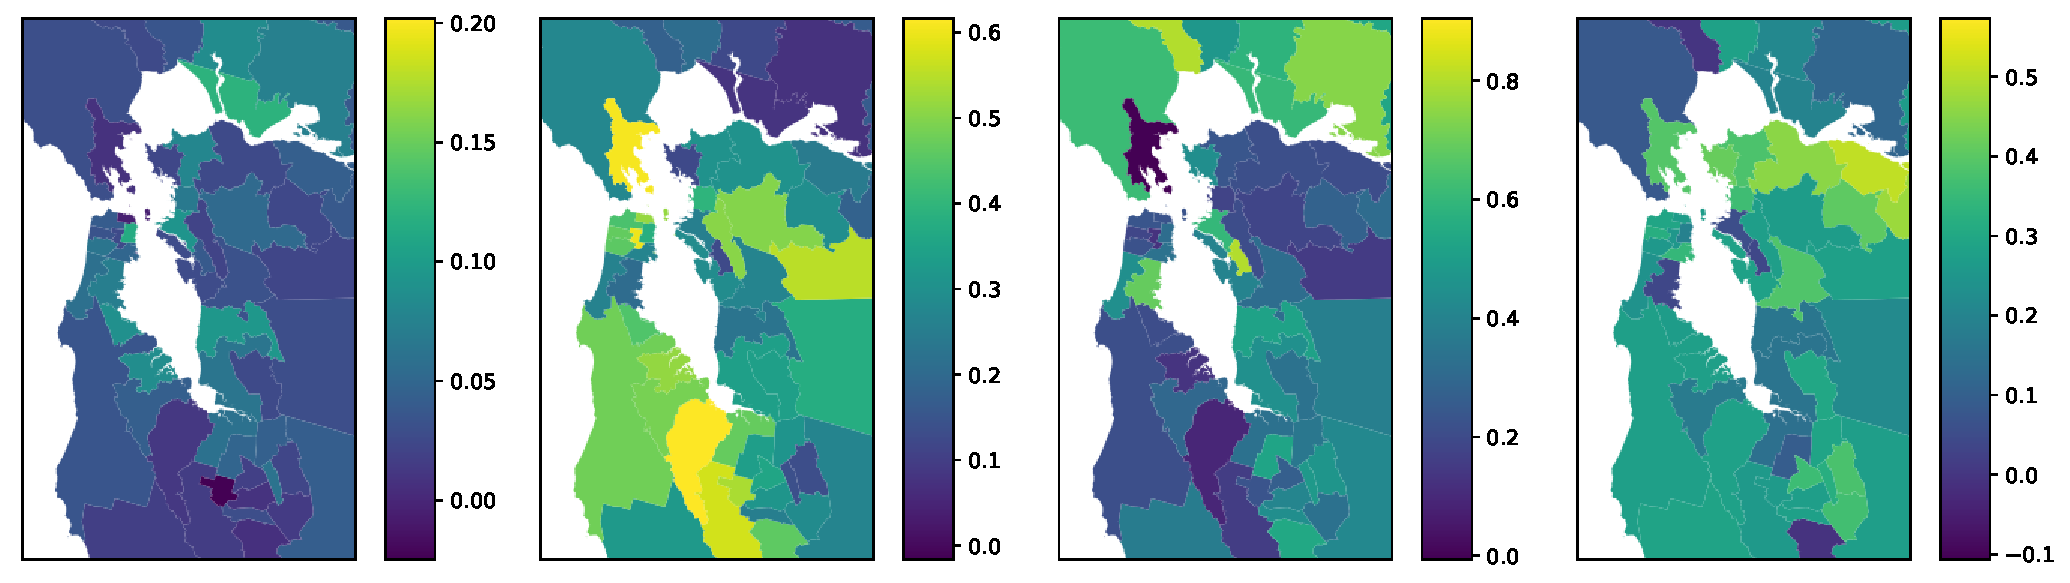
\includegraphics[width=0.9\linewidth]{income_lam_sf}
}
\only<7>{
\centering

\hspace{1cm} 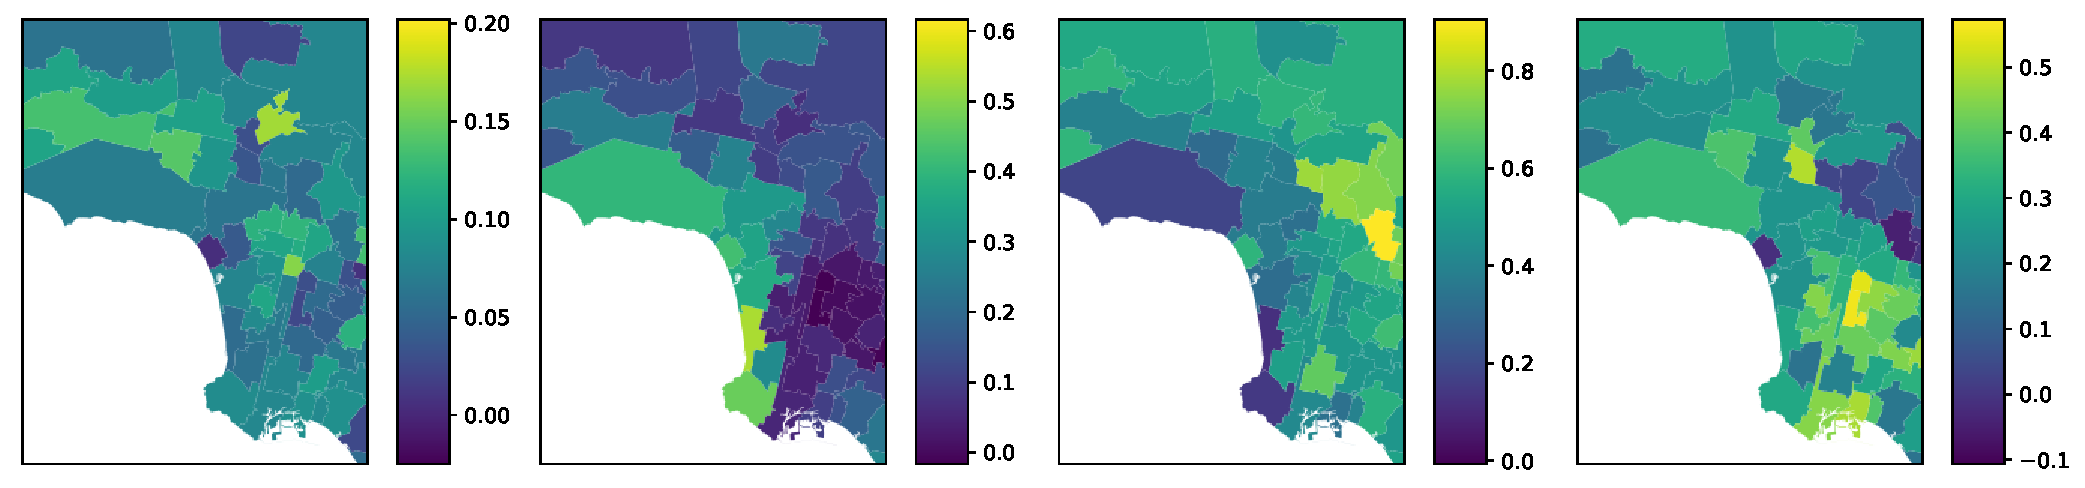
\includegraphics[width=0.9\linewidth]{income_lam_la}
}

\end{frame}


\begin{frame}{Conclusions}

\textbf{Normalized Latent Random Measures}

\medskip

\begin{itemize}[<+->]
	\setlength{\itemsep}{1.2em}
	
	\item A framework for exploring difference in distribution across groups of data
	
	\item Scalable to ``big data'' settings
	
	\item Interpretability through post-processing
	\begin{itemize}
		\item Latent measures $\longrightarrow$ \textbf{latent common traits} across populations
		\item $\Lambda$ $\longrightarrow$  to explore the variability
	\end{itemize}
	
	\item Trade-off between analytical tractability and algorithmic efficiency / scalability
	\begin{itemize}
		\item Posterior (of the $\mu^*_h$'s) is not a CoRM. No marginal distribution in close form.
		\item Prior elicitation carried out case-by-case
	\end{itemize}
	
\end{itemize}

\end{frame}


\begin{frame}{References}

Birgin and Mart{\'\i}nez. \emph{Practical augmented Lagrangian methods for constrained optimization}. SIAM 2014

\medskip
França, Barp, Girolami, and Jordan. \emph{Optimization on manifolds: A symplectic approach}.  arXiv 2107.11231

\medskip
Griffin and Leisen. \emph{Compound Random Measures and their use in Bayesian nonparametrics}. JRSSB 2017

\medskip
Griffin, Kolossiatis, and Steel. \emph{Comparing distributions by using dependent normalized random-measure mixtures}. JRSSB 2013

\medskip
Lijoi, Nipoti, and P{\"u}nster. \emph{Bayesian inference with dependent normalized completely random measures}. Bernoulli 2014

\medskip
Poworoznek, Ferrari, and Dunson. \emph{Efficiently resolving rotational ambiguity in bayesian matrix sampling with matching}. arXiv:2107.13783

\medskip
Teh, Jordan, Beal, and Blei. \emph{Hierarchical Dirichlet Processes}. JASA (2006)

\end{frame}

\addtocounter{framenumber}{-7}

\appendix

\begin{frame}{Theoretical results}

\begin{theorem}\label{teo:expectation}
    Let $(\mu^*_1, \ldots, \mu^*_H)$ be a CoRM with i.i.d. scores. Denote with $\mathcal{L}_m(u) := \E[e^{-u m}]$ the Laplace transform of the scores' distribution and with $\kappa_m(u, n) := \E[e^{-u m} m^n]$.
    Then for all measurable $A \subset \Theta$
    \begin{multline*}
        \E[\ptilde_j(A)] = \\ \alpha(A) \sum_{h=1}^H \int \E\left[ \lambda_{jh}  \psi_{\rho}(u\lambda_{j1}, \ldots, u \lambda_{jH}) \int_{\R_+} z \prod_{k \neq h} \mathcal{L}_m(u \lambda_{jk} z) \kappa_m(u \lambda_{jh} z, 1) \nu^*(\dd z) \right] \dd u 
    \end{multline*}
    where $\psi_{\rho}$ is the Laplace functional of $(\mu^*_1, \ldots, \mu^*_H)$ (evaluated at the constant functions $u\lambda_{j1}, \ldots, u \lambda_{jH}$).
  \end{theorem}
\end{frame}


\begin{frame}{Theoretical results, cont'd}


\begin{proposition}
The following expression holds.
    \begin{multline*}
        \Cov\left[\mutilde_j(A), \mutilde_\ell(B)\right]  =  \\ \sum_{h, k} \E[\lambda_{jh} \lambda_{\ell k}] \Cov (\mu^*_h(A), \mu^*_k(B)) + \Cov(\lambda_{jh}, \lambda_{\ell k}) \E[\mu^*_h(A) \mu^*_k(B)] 
    \end{multline*}
    If the $\lambda_{jh}$'s have the same marginal distribution, the $\mu^*_h$'s have the same marginal distribution, $\lambda_j = (\lambda_{j1}, \ldots, \lambda_{jH})$ and $\lambda_\ell$ (defined analogously) are independent, $\E[\lambda_{jh} \lambda_{\ell h}] = \kappa$,  $\Cov(\lambda_{jh}, \lambda_{\ell h}) = \rho$ for all $j, \ell, h$, then:
    \begin{multline*}
	\Cov\left[\mutilde_j(A), \mutilde_\ell(B)\right]  =  \\ \Cov(\mu^*_1(A), \mu^*_1(B)) \kappa H + m^*_1(A) m^*_1(B) \rho H + \sum_{h \neq q} \bar \lambda_{11}^2  \Cov(\mu^*_h(A), \mu^*_k(B))
\end{multline*}
%    where $\bar{\lambda}_{jh} := \E[\lambda_{jh}]$ and  $m^*_h(A) = \E[\mu^*_h(A)]$.
%
%Finally, if in addition the $\mu^*_h$'s are independent, the latter sum disappears
\end{proposition}
\end{frame}



\begin{frame}{Prior Elicitation, Invalsi dataset}

$\mbox{Corr}(\mutilde_j(A), \mutilde_\ell(A))$ for $H=4, 8, 16$ when $a_1 = 2.5$ and $\phi=2$.

\vspace{0.5cm}

\begin{center}
	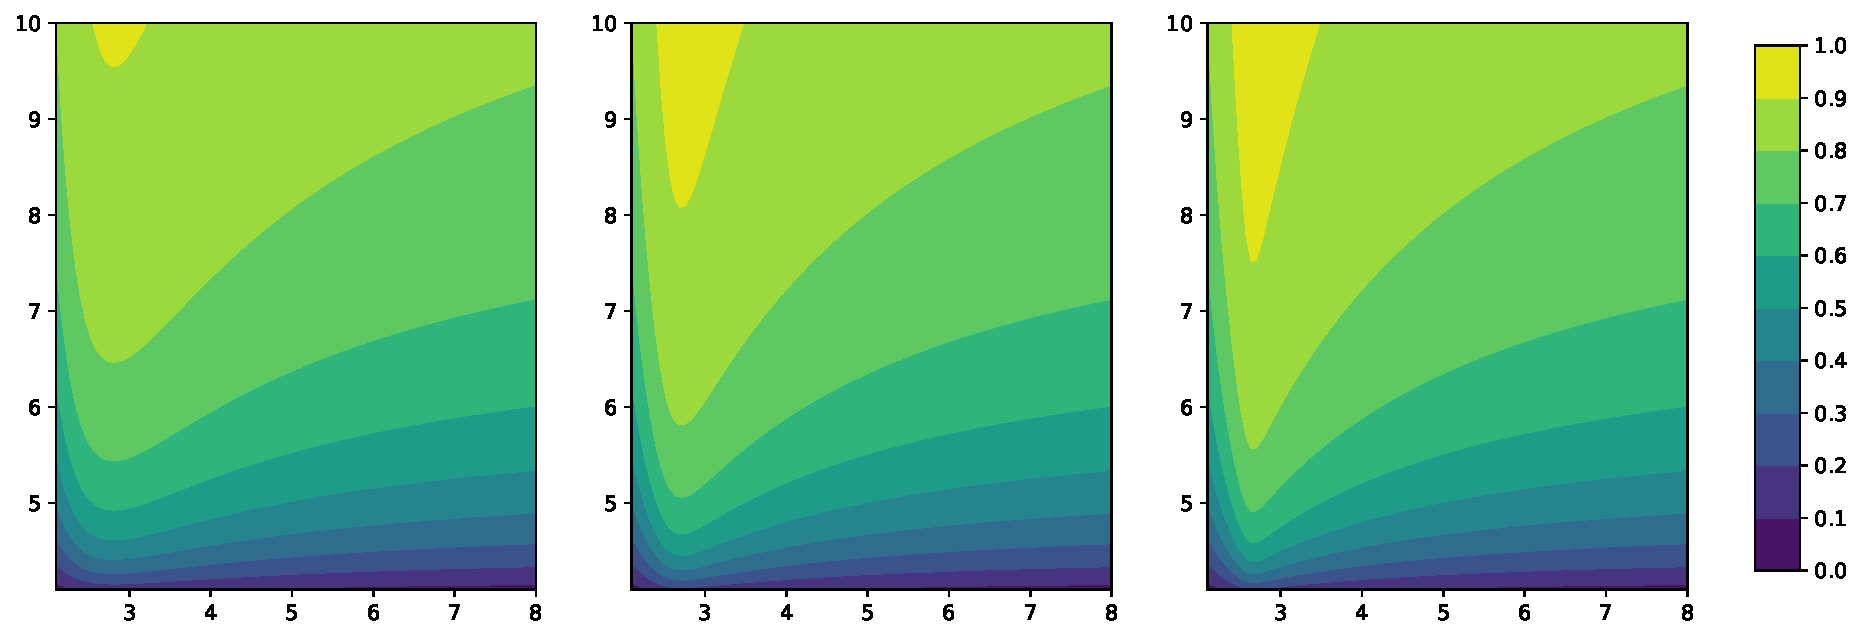
\includegraphics[width=0.9\linewidth]{corr_mgp} \\
	$x$-axis: $a_2$, $y$-axis: $\nu$.
\end{center}

\pause

\medskip

We set as default $a_2 = 3$ and $\nu=5$.
\end{frame}


\begin{frame}{Prior Elicitation, US Income}

$\mbox{Corr}(\mutilde_j(A), \mutilde_\ell(A))$ for $H=4, 8, 16$ for $j \sim \ell$ (first row) and $j$ far apart from $\ell$ (second) row

\begin{center}
	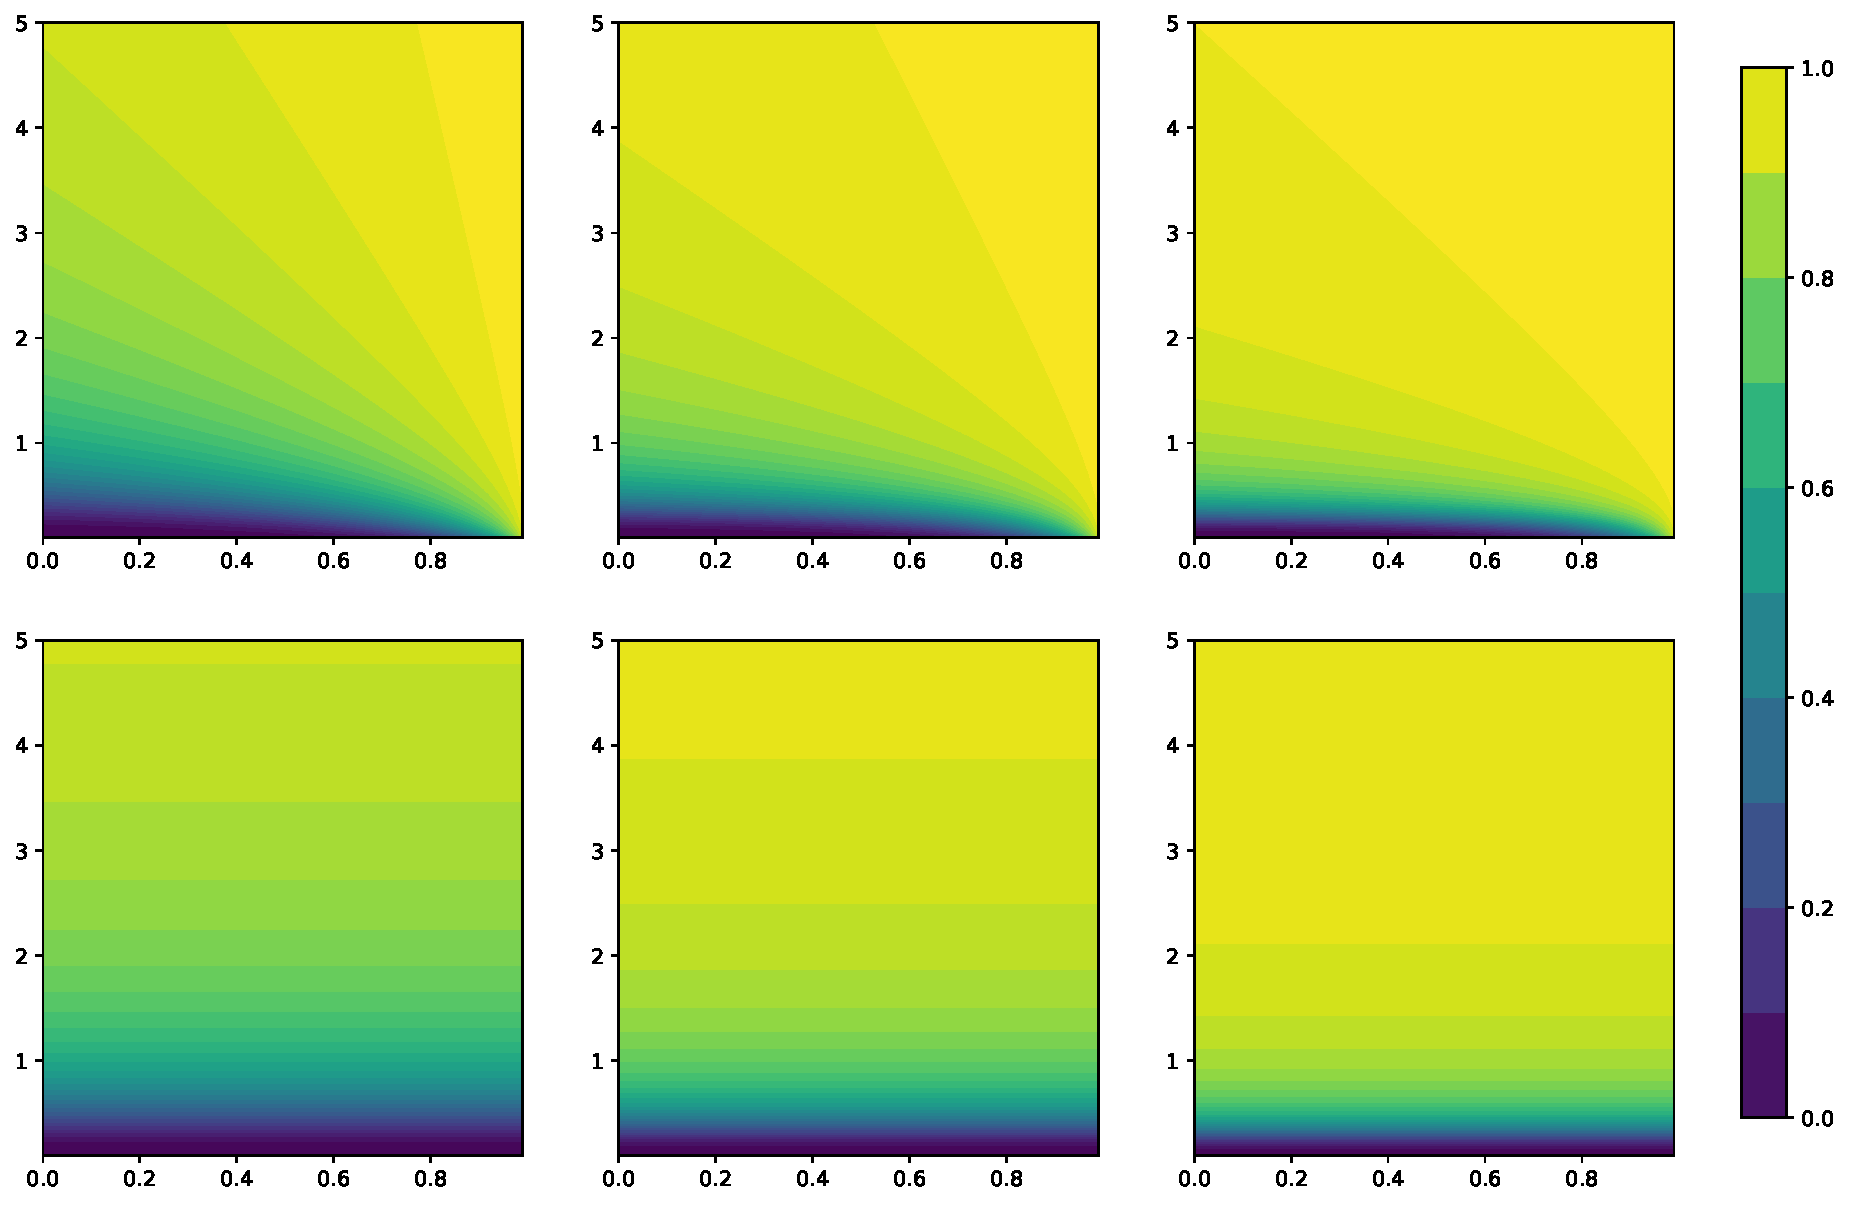
\includegraphics[width=0.6\linewidth]{corr_lgmrf} \\
	$x$-axis: $\rho$, $y$-axis: $\tau$.
\end{center}

\end{frame}


\begin{frame}{Postprocessing Algorithm: RALM}
\textbf{Input}: Starting point $Q$, initial values $\rho$, $\gamma_{j}$, target threshold $\varepsilon^*$, initial threshold $\varepsilon$

\bigskip

While $\varepsilon \leq \varepsilon^*$; $\|Q - Q^\prime\| \leq \varepsilon$, \textbf{repeat}:

\bigskip
\begin{enumerate}
	\setlength{\itemsep}{1.5em}
	\item $Q = Q^\prime$ 
	\item	solve $Q^\prime = \arg\min_Q \mathcal L_\rho(Q, \gamma)$ for fixed $\rho, \gamma$ with theshold $\varepsilon$  	
	\item $\gamma_j = \gamma_j + \rho c_j(Q^\prime)$
	\item $\rho = 0.9 \rho$ $\varepsilon = \max\{\varepsilon^*, 0.9 \varepsilon\}$
	\end{enumerate}
\end{frame}



\begin{frame}{Postprocessing Algorithm: Inner Optimization}
\textbf{Input}: Starting point $Q, P$, momentum $\tau$, stepsize $s$, threshold $\varepsilon$

\bigskip

While $\|Q - Q^\prime\| \leq \varepsilon$, \textbf{repeat}:

\bigskip
\begin{enumerate}
	\setlength{\itemsep}{1.5em}
	\item $P = \tau \left(P - s \Pi_{\mathfrak {sl}(H)}(\partial_Q \mathcal L_\rho(Q, \gamma), Q)\right)$
	\item	$Q = Q \exp_m(\chi P )$, $\chi = \cosh(- \log \tau)$
	\item	$P = \tau \left(P - s \Pi_{\mathfrak {sl}(H)}(\partial_Q \mathcal L_\rho(Q, \gamma), Q)\right)$ 
\end{enumerate}
\end{frame}

\begin{frame}{Simulation on Area  Referenced data}

Data on a $\sqrt{g} \times \sqrt{g}$ regular lattice.
\[
	y_{j,i} \iid w_{j1} \mathcal N(-5, 1) + w_{j2} \mathcal N(0, 1) + w_{j3} \mathcal N(5, 1)
\]
\only<1>{
\[
    (w_{j1}, w_{j2}, w_{j3}) = \left(e^{\widetilde{w}_{j1}}, e^{\widetilde{w}_{j2}}, 1 \right) \big/ \left( 1 + e^{\widetilde{w}_{j1}} + e^{\widetilde{w}_{j2}} \right)
\]
where 
\[
    \widetilde{w}_{j1} =  3(x_j - \bar x) + 3(y_j - \bar y), \quad \widetilde{w}_{j2} =  -3(x_j - \bar x) - 3(y_j - \bar y)
\]
and $(\bar x, \bar y)$ denote the center of the lattice. 
}

\only<2>{
\begin{center}
    \centering
    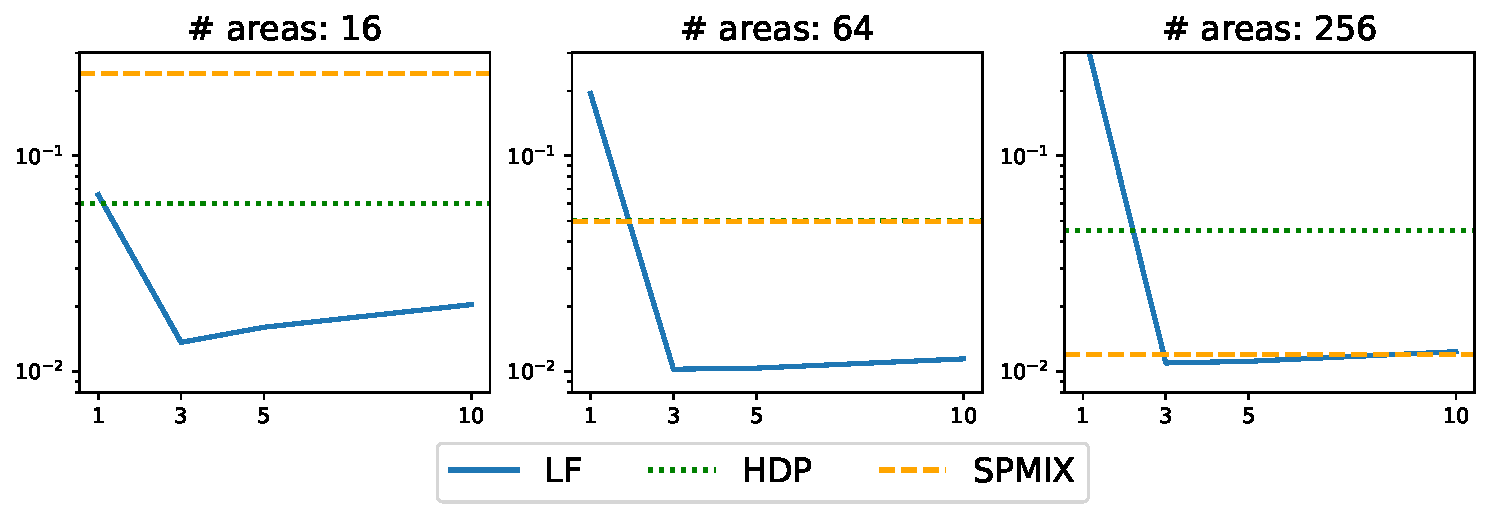
\includegraphics[width=\linewidth]{spatial_kl.pdf}
    Average Kullback--Leibler divergence (across all the groups)  
\end{center}
}
\end{frame}

\end{document}